\chapter{The DCT: recipes for pictures}\label{ch:dct}

\section{The intuition}

Think of a sound. A chord on a piano \emph{looks} like a complicated wiggly line, but it is really three or four pure notes added together. Writing down ``note A at volume 3, note C at volume 1'' is much shorter than writing down thousands of samples of the wiggly line.

Pictures work the same way. Any $8\times8$ tile can be built by adding up 64 fixed \emph{pattern tiles}, each scaled by some amount. The 64 patterns are shown below: the top-left is a flat grey (no variation), moving right adds more vertical stripes, moving down adds more horizontal stripes, and the bottom-right is a fine checkerboard.

\begin{figure}[h]
\centering
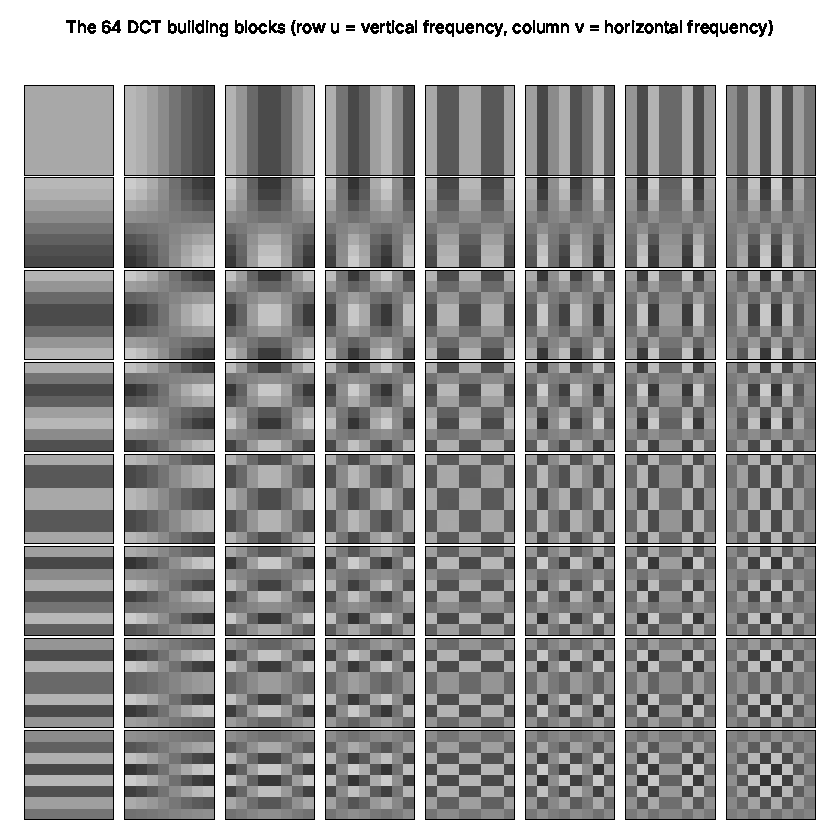
\includegraphics[width=0.62\textwidth]{figures/dct_basis.pdf}
\caption{The 64 building blocks of the $8\times8$ DCT. Any tile is a weighted sum of these. Weights near the top-left (smooth patterns) are usually big, weights near the bottom-right (fine detail) are usually tiny.}
\end{figure}

The \textbf{DCT} (Discrete Cosine Transform) is the machine that answers ``how much of each pattern is in this tile?'' It outputs 64 numbers, one per pattern, called \emph{coefficients}. The inverse DCT adds the patterns back up and returns the tile. Nothing is lost in this step; it is just a change of description.

\begin{plain}
\textbf{Why bother?} Because for natural pictures, after the change of description, most of the 64 numbers are close to zero. The energy is \emph{compacted} into a few coefficients. The next step can then round the small ones to exactly zero without anyone noticing.
\end{plain}

\begin{figure}[h]
\centering
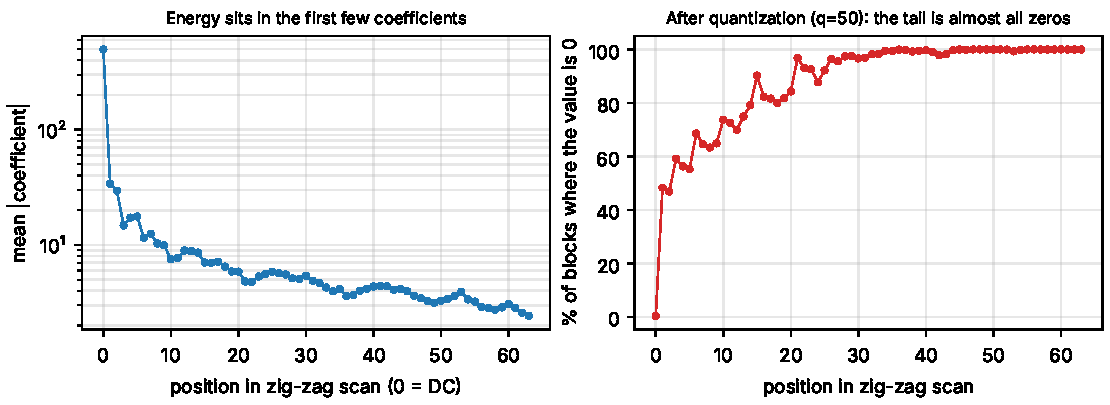
\includegraphics[width=0.95\textwidth]{figures/energy_compaction.pdf}
\caption{Left: average size of each coefficient (in zig-zag order, Chapter~\ref{ch:zigzag}) over all tiles of the cameraman: the first few dominate by orders of magnitude. Right: after quantization at quality~50, the share of tiles in which each position is exactly zero.}
\end{figure}

\section{The formula, one dimension first}

Take 8 numbers $x_0,\dots,x_7$ (one row of a tile). The DCT produces 8 coefficients
\begin{equation}
X_u \;=\; \alpha(u)\sum_{x=0}^{7} x_x \cos\!\Big(\frac{(2x+1)\,u\,\pi}{16}\Big),\qquad
\alpha(0)=\sqrt{\tfrac18},\quad \alpha(u>0)=\sqrt{\tfrac28}=\tfrac12 .
\end{equation}

How to read it:
\begin{itemize}
\item $u$ is the \emph{frequency}: how many half-waves of a cosine fit across the 8 samples. $u=0$ is a flat line, $u=1$ is one slow half-wave from bright to dark, $u=7$ wiggles up and down almost every sample.
\item The sum multiplies the data by that cosine and adds it up. If the data looks like the cosine, the sum is large (the pattern is ``present''); if not, positive and negative terms cancel and the sum is near zero.
\item The factor $\alpha(u)$ is only a scaling constant that makes the transform \emph{orthonormal}, explained below.
\item The odd-looking $(2x+1)/16$ means each sample is evaluated at the \emph{centre} of its pixel. This choice (the ``type-II'' DCT) is what makes JPEG's tiles behave well at their borders.
\end{itemize}

\section{Two dimensions: do rows, then columns}

For a tile $X$ (an $8\times8$ array), the 2D DCT has frequency $u$ vertically and $v$ horizontally:
\begin{equation}
Y_{uv} \;=\; \alpha(u)\alpha(v)\sum_{x=0}^{7}\sum_{y=0}^{7} X_{xy}\cos\!\Big(\tfrac{(2x+1)u\pi}{16}\Big)\cos\!\Big(\tfrac{(2y+1)v\pi}{16}\Big).
\end{equation}
This is 64 outputs, each a sum of 64 terms: $4096$ multiply-adds. But the formula \emph{factorizes}, so we can do a 1D DCT on every column, then a 1D DCT on every row. In matrix language, define the $8\times8$ matrix $C$ with entries $C_{ux}=\alpha(u)\cos\big(\tfrac{(2x+1)u\pi}{16}\big)$. Then
\begin{equation}
\boxed{\,Y \;=\; C\,X\,C^{\!\top}\,}\qquad\text{and the inverse is}\qquad \boxed{\,X \;=\; C^{\!\top}\,Y\,C\,}
\end{equation}
Each matrix product costs $8\cdot8\cdot8=512$ multiply-adds, two of them make \textbf{1024}, a 4$\times$ saving over the double sum. (Dedicated fast algorithms such as AAN need only roughly 5 multiplications and 29 additions per 8-point transform; our code does not use them, on purpose, for clarity.)

\subsection{Why the inverse is just the transpose}

The rows of $C$ are the 8 cosine patterns scaled by the $\alpha$'s so that each row has length 1 and any two different rows are perpendicular (dot product 0). That is exactly the statement
\begin{equation}
C\,C^{\!\top} = I \quad\Longrightarrow\quad C^{-1}=C^{\!\top}.
\end{equation}
A matrix with this property is called \emph{orthonormal} (a ``rotation'' in 8 dimensions). The test \code{dct\_matrix\_is\_orthonormal} checks this numerically. Two useful consequences:

\begin{enumerate}
\item \textbf{Perfect reconstruction.} Apply $C$ then $C^{\top}$ and you get the tile back (up to $10^{-13}$ floating-point noise).
\item \textbf{Energy conservation (Parseval).} Sum of squares is unchanged: $\sum Y_{uv}^2=\sum X_{xy}^2$. Proof in one line, with $\|\cdot\|_F$ the sum of squares:
\[
\|Y\|_F^2=\operatorname{tr}\!\big(C X C^{\!\top} C X^{\!\top} C^{\!\top}\big)=\operatorname{tr}\!\big(C X X^{\!\top} C^{\!\top}\big)=\operatorname{tr}\!\big(X X^{\!\top}\big)=\|X\|_F^2 .
\]
This is how we later predict pixel-domain error from coefficient-domain error, and why no single coefficient can exceed $\sqrt{64\cdot128^2}=1024$.
\end{enumerate}

\subsection{A sanity check you can do by hand}

For a perfectly flat tile of value $a$: only $Y_{00}$ is non-zero and equals $8a$ (the test \code{dct\_flat\_block\_has\_only\_dc\_equal\_to\_8\_times\_value}). The DC coefficient is always \emph{8 times the tile's average}. Our example tile after the DCT (rounded to integers for display):
\[
\begin{pmatrix}
551 & 1 & 10 & 0 & 2 & 0 & 0 & 1 \\
78 & 2 & -11 & 0 & -1 & -2 & 1 & -1 \\
-59 & -1 & 6 & 1 & 2 & 0 & -2 & 1 \\
43 & -2 & -5 & -1 & -1 & 0 & 1 & 0 \\
-28 & 0 & 6 & 2 & 0 & 0 & -1 & 0 \\
13 & 1 & -3 & -4 & 1 & 0 & 1 & 0 \\
-7 & 1 & 3 & 2 & 0 & 0 & 1 & 0 \\
4 & -2 & -2 & 1 & 1 & -2 & -2 & 1
\end{pmatrix}
\]
Look at the top-left entry (the DC, brightness of the whole tile) and how quickly the magnitudes fall away towards the bottom-right.

\section{Why the DCT and not the Fourier transform?}

\begin{itemize}
\item \textbf{Real numbers only.} The DFT produces complex numbers (two values per frequency). The DCT produces one real number per frequency.
\item \textbf{No false edges at the borders.} The DFT implicitly repeats the tile periodically; a tile that goes from dark on the left to bright on the right becomes a sawtooth with a sudden jump, which smears energy over all frequencies. The DCT implicitly \emph{mirrors} the tile at its borders (a triangle wave instead), so there is no jump, and the energy stays in a few low-frequency coefficients.
\end{itemize}

\section{The code}

The matrix is built once from the formula:
\lstinputlisting{snippets/code_dct_matrix.cpp}
and the forward transform is exactly the two matrix products $T=CX$, $Y=TC^{\top}$:
\lstinputlisting{snippets/code_dct_forward.cpp}

\begin{plain}
\textbf{Reading the code.} \code{in} and \code{out} are 64 numbers in row-major order (index $=8\cdot{\rm row}+{\rm col}$). The first double loop computes one column-transform output $T[u][y]$ as a dot product of row $u$ of $C$ with column $y$ of the tile. The second does the same along rows. It uses \code{double}, so rounding noise is about $10^{-13}$; Chapter~\ref{ch:numerics} shows why that is far more than enough.
\end{plain}

The function \code{forwardDCT8x8Naive} in the same file is the 4-fold sum straight from the textbook. It is slow and exists only so that the tests can prove the fast matrix version computes the same thing (agreement to $10^{-10}$ on 50 random tiles).

\begin{sound}
``The DCT is an orthonormal change of basis from pixel values to 64 cosine patterns. Orthonormal gives me two things for free: the inverse is the transpose, and squared error is preserved, so I can reason about distortion in either domain. I implemented it as $CXC^{\top}$, 1024 multiply-adds per tile, and validated it against the textbook double sum.''
\end{sound}
